\documentclass[a4paper,12pt]{article}
\usepackage[T1]{fontenc}
\usepackage{ninecolors}
\usepackage{booktabs}
\usepackage{caption}
\usepackage{tabularray}
\usepackage{geometry}
\usepackage{siunitx}
\usepackage{pdfpages}
\usepackage{hyperref}
\hypersetup{
  colorlinks=true,
  linkcolor=blue,
  filecolor=magenta,
  urlcolor=cyan,
  pdftitle={Elements: Modulation},
  pdfpagemode=FullScreen,
}

\begin{document}
\begin{titlepage}
  \vspace*{\stretch{1.0}}
  \begin{center}
    \Large\textbf{Elements: Modulation}\\
    \large{Effect Design Workshop by Pedal Markt}
  \end{center}
  \vspace*{\fill}
  \begin{center}
    \today
  \end{center}
\end{titlepage}

\section{Summary}

Elements: Modulation is the second event in the series of
our effect-design workshops. The goal is to give you all the
tools, knowledge and a bit of intuition to start designing
effects yourself!

The workshop covers:

\begin{itemize}
  \item How modulation effects work and what parts they
    consist of;
  \item Sources, transformations and destinations that can
    we use can use CV (Control Voltage) with;
  \item Adding CV to almost any circuit.
\end{itemize}

\section{Voltage Standard}\label{voltage}

All the workshop boards use \SI{4.5}{\V} reference voltage
as a virtual ground. Votages below \SI{4.5}{\V} are
considered negative, above \SI{4.5}{\V} --- positive.
Circuits \textit{can} accepts and output control voltage in
the range \SI{0}{\V}-\SI{9}{\V}, but an effective range is
considered to be \SI{2}{\V}-\SI{7}{\V} (\SI{5}{\V} range
centered around \SI{4.5}{\V}).

That voltage standard makes sense for effect pedals, but
some of the circuits are a bit more complex than they would
be in a triple voltage rail system like Eurorack. My
personal observation is that the world is moving on to
dual rail systems, so learning to work with them might
benefit you in any case.

\section{Included modules}

Here's a list of modules included with the worskshop and
their functions:

\begin{itemize}
  \item \hyperref[sec:attvert]{\textbf{AttVert}} --- Two
    attenuverters with offset. Can be used as a DC voltage
    source or to scale and shift an incoming signal;

  \item \hyperref[sec:longwave]{\textbf{Longwave}} --- LFO
    module based on
    \href{https://electricdruid.net/datasheets/STOMPLFODatasheet.pdf}{StompLFO}
    digital chip;

  \item \hyperref[sec:mag]{\textbf{Mag}} --- 2x exponential
    and 1x linear VCA module based on
    \href{https://www.soundsemiconductor.com/downloads/ssi2164datasheet.pdf}{SSI2164}
    analog 4-in-1 VCA chip;

  \item \hyperref[sec:demod]{\textbf{Demod}} --- Envelope
    follower and peak detector.
\end{itemize}

\pagebreak

\section{AttVert}\label{sec:attvert}

AttVert is two attenuverters with offset function on a
single board.

\begin{itemize}
  \item Schematic PDF:
    \href{https://github.com/flpvsk/pedalmarkt-docs/tree/main/elements2-modulation-docs/include}{GitHub}

  \item KiCad project:
    \href{https://github.com/flpvsk/pt-workshop/tree/main/attenuverters}{GitHub}
\end{itemize}


\begin{table}[h!]
  \caption{AttVert Pinout}
  \centerline{
    \begin{tblr}{
      hlines,
      vlines,
      rows={ht=1.2em},
      row{1}={bg=gray3,fg=white},
      colspec={cccX[l]}
    }
      \textbf{Pin}
      & \textbf{Name}
      & \textbf{Type}
      & \textbf{Description}
      \\
      1 & In1 & In & Input of the first attenuverter, defaults
      to \SI{4.5}{\V} when unconnected
      \\
      2 & GND & Pwr & Ground
      \\
      3 & Out1 & Out & Output of the first attenuverter
      \\
      4 & 9V0 & Pwr & \SI{9}{\V} power
      \\
      5 & GND & Pwr & Ground
      \\
      6 & 4V5 & Ref & \SI{4.5}{\V} reference
      \\
      7 & In2 & In & Input of the second attenuverter, defaults
      to \SI{4.5}{\V} when unconnected
      \\
      8 & GND & Pwr & Ground
      \\
      9 & Out2 & Out & Output of the second attenuverter
    \end{tblr}
  }
\end{table}

\pagebreak

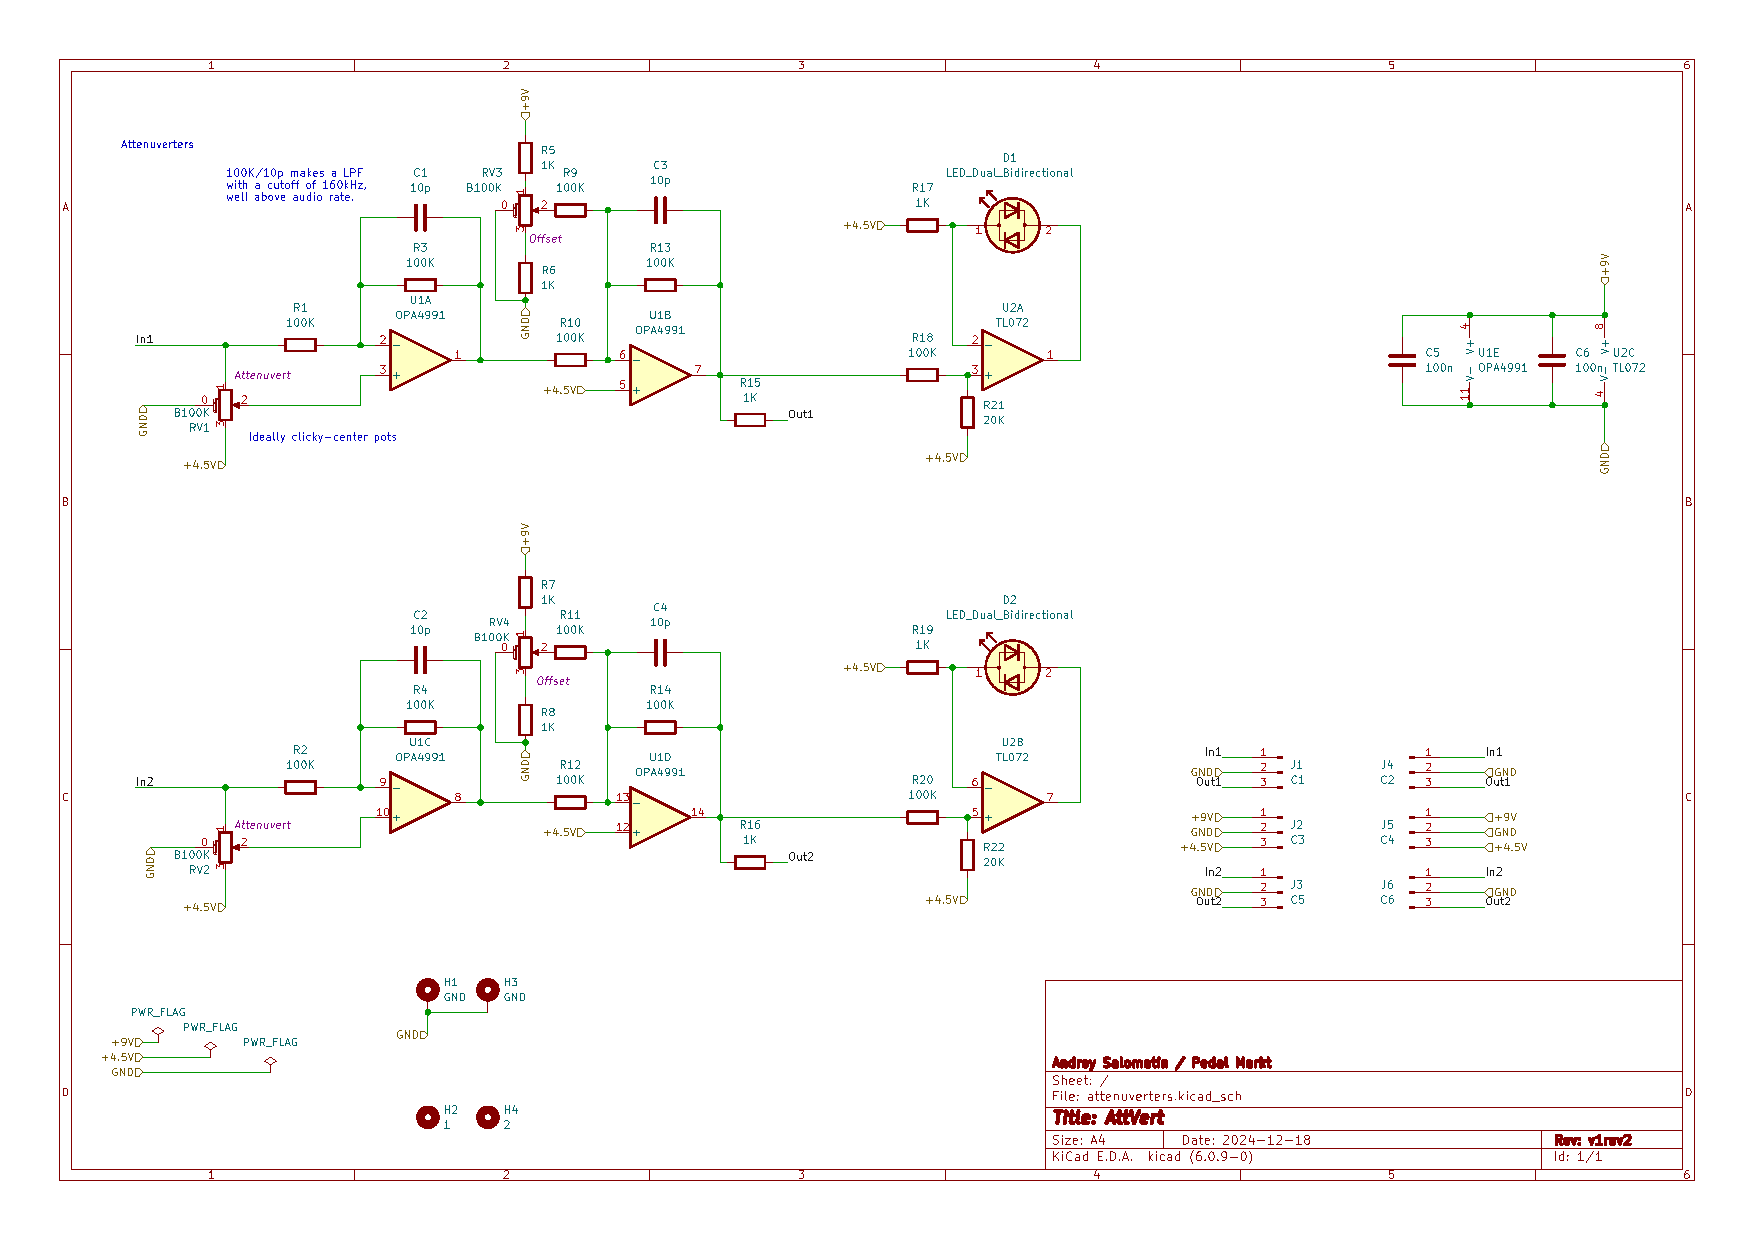
\includepdf[pages=-,landscape=true]{include/attvert-v1rev2.pdf}

\section{Longwave}\label{sec:longwave}

Longwave is an LFO module with
\href{https://electricdruid.net/datasheets/STOMPLFODatasheet.pdf}{StompLFO}
digital chip at its core.

StompLFO is a PIC microcontroller programmed by
\href{https://electricdruid.net}{Electric Druid} to produce
\href{https://en.wikipedia.org/wiki/Pulse-density_modulation}{Pulse-Density
Modulated} signal, effectively a square-wave that changes
very fast, that then gets filtered by an active low-pass on
the board to produce an analog voltage signal at the output.

StompLFO is a 5V-chip, that means that it's powered by and
has an analog input limit of \SI{5}{V}. The rest of the
circuitry in Longwave is shifting, scaling and limiting the
range of the incoming CV to match the
\hyperref[voltage]{Voltage Standard} the other boards
follow.


\begin{itemize}
  \item Schematic PDF:
    \href{https://github.com/flpvsk/pedalmarkt-docs/tree/main/elements2-modulation-docs/include}{GitHub}

  \item KiCad project:
    \href{https://github.com/flpvsk/pt-workshop/tree/main/lfo-board}{GitHub}
\end{itemize}

\pagebreak

\begin{table}[h!]
  \caption{Longwave Pinout}
  \centerline{
    \begin{tblr}{
      hlines,
      vlines,
      rows={ht=1.2em},
      row{1}={bg=gray3,fg=white},
      colspec={cccX[l]}
    }
      \textbf{Pin}
      & \textbf{Name}
      & \textbf{Type}
      & \textbf{Description}
      \\
      1 & 9V0 & Pwr & \SI{9}{\V} power
      \\
      2 & GND & Pwr & Ground
      \\
      3 & 4V5 & Ref & \SI{4.5}{\V} reference
      \\
      4 & 5V0 & Pwr/Out & \SI{5}{\V} reference generated by
      the board
      \\
      5 & GND & Pwr & Ground
      \\
      6 & Out & Out & Output
      \\
      7 & GND & Pwr & Ground
      \\
      8 & Sync & In & Syncs the LFO to the low-to-high
      transition of an incoming square wave
      \\
      9 & Tap & In & Syncs the LFO to the high-to-low
      transition of an incoming square wave
      \\
      10 & Vfreq & In & Frequency CV
      \\
      11 & Vof & In & Offset CV
      \\
      12 & GND & Pwr & Ground
      \\
      13 & Vform & In & Waveform CV
      \\
      14 & Vdepth & In & Depth CV
      \\
      15 & GND & Pwr & Ground
    \end{tblr}
  }
\end{table}

\pagebreak

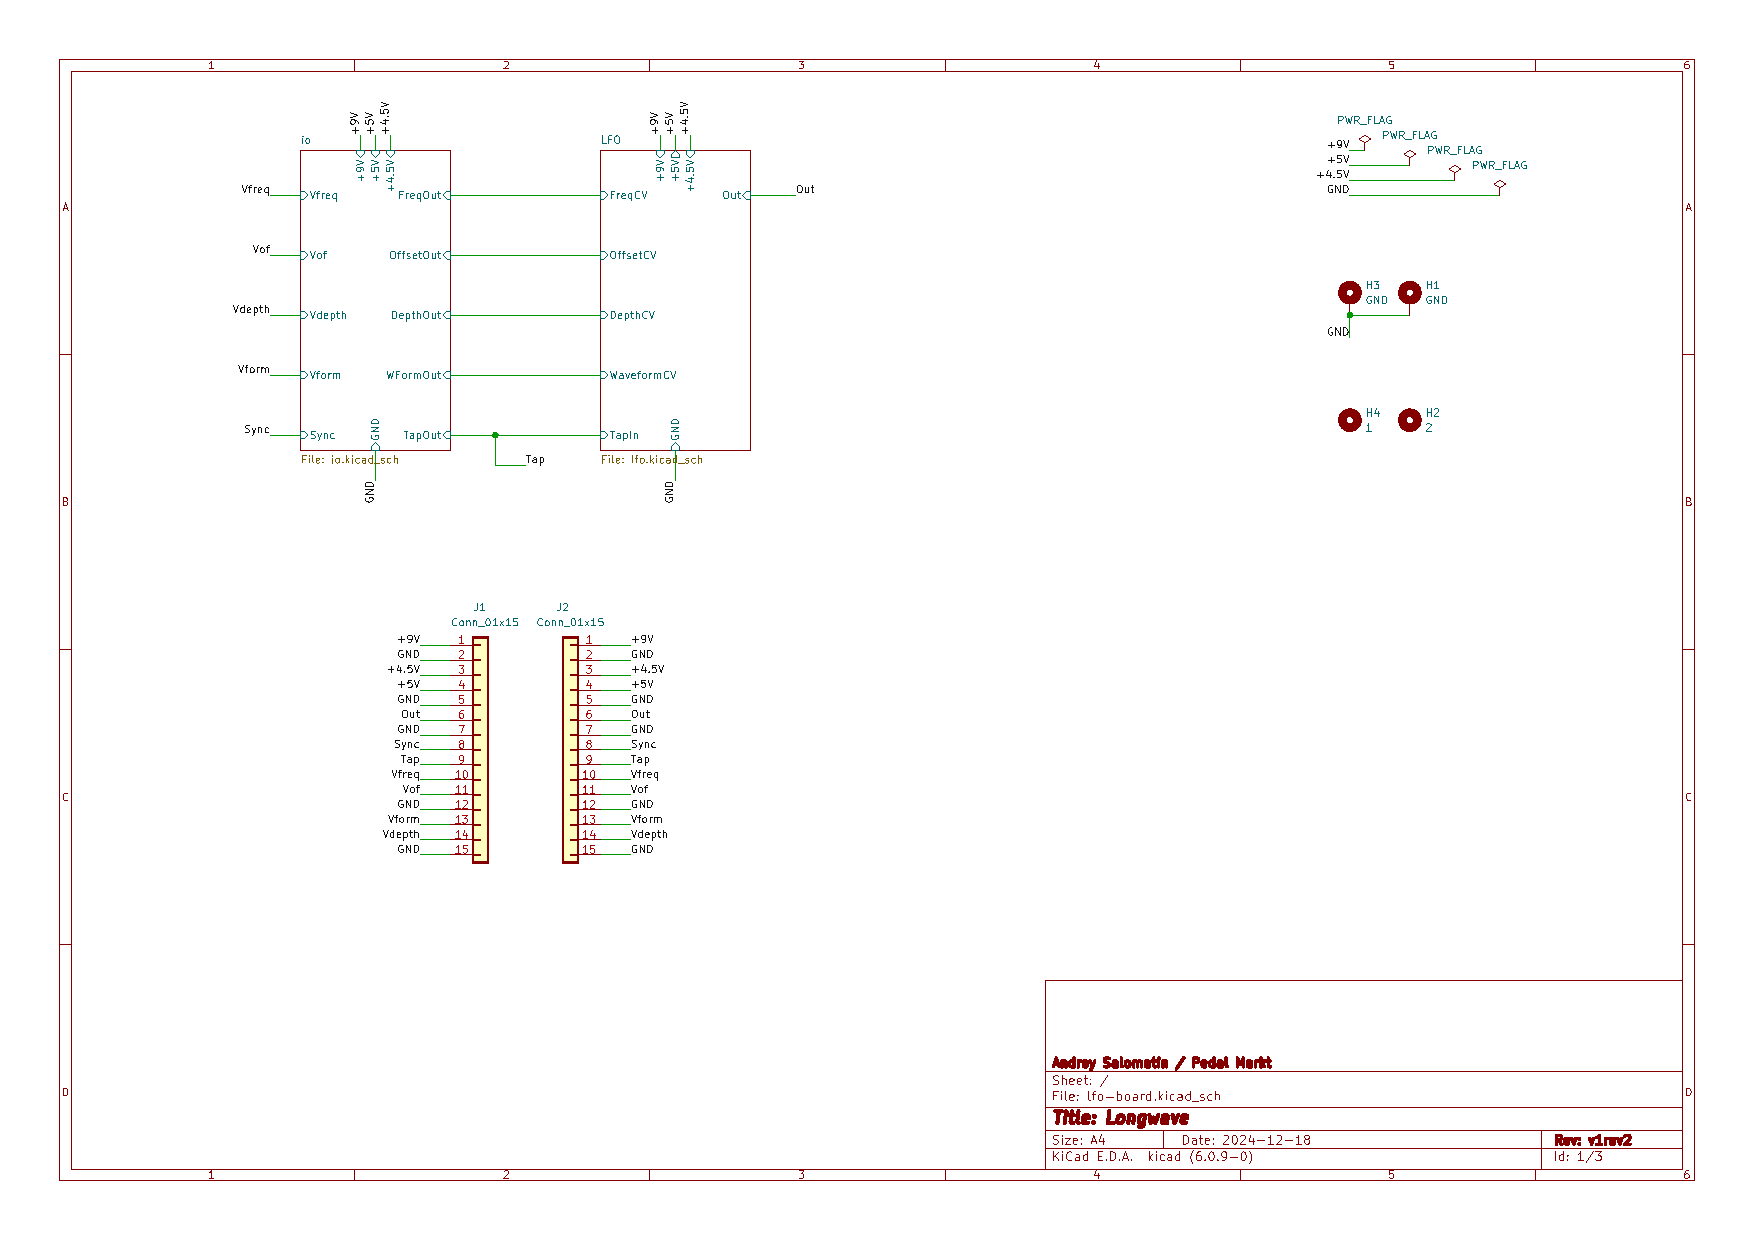
\includepdf[pages=-,landscape=true]{include/longwave-v1rev2.pdf}

\section{Mag}\label{sec:mag}

Mag is three VCAs on a single board. VCA1 and VCA2 have
exponential response. VCA3 has a linear response. All the
VCAs can be used to attenuate both DC and AC coupled signals
centered around the virtual ground of \SI{4.5}{V}.

The board is based around the
\href{https://www.soundsemiconductor.com/downloads/ssi2164datasheet.pdf}{SSI2164}
analog 4-in-1 VCA chip. The VCAs on the chip all have
exponential response and there's a bit of extra circuitry
added to make one of them linear.

The rest of the board's circuitry is scaling, shifting and
limiting incoming signals to match the chip's working
ranges.

\begin{itemize}
  \item Schematic PDF:
    \href{https://github.com/flpvsk/pedalmarkt-docs/tree/main/elements2-modulation-docs/include}{GitHub}

  \item KiCad project:
    \href{https://github.com/flpvsk/pt-workshop/tree/main/vca-board}{GitHub}
\end{itemize}

\pagebreak

\begin{table}[h!]
  \caption{Mag Pinout}
  \centerline{
    \begin{tblr}{
      hlines,
      vlines,
      rows={ht=1.2em},
      row{1}={bg=gray3,fg=white},
      colspec={cccX[l]}
    }
      \textbf{Pin}
      & \textbf{Name}
      & \textbf{Type}
      & \textbf{Description}
      \\
      1 & 9V0 & Pwr & \SI{9}{\V} power
      \\
      2 & GND & Pwr & Ground
      \\
      3 & 4V5 & Ref & \SI{4.5}{\V} reference
      \\
      4 & GND & Pwr & Ground
      \\
      5 & CV1 & In & CV input for the first VCA
      \\
      6 & In1 & In & Input for the first VCA
      \\
      7 & GND & Pwr & Ground
      \\
      8 & Out1 & Out & Output of the first VCA
      \\
      9 & GND & Pwr & Ground
      \\
      10 & CV2 & In & CV input for the second VCA
      \\
      11 & In2 & In & Input for the second VCA
      \\
      12 & GND & Pwr & Ground
      \\
      13 & Out2 & Out & Output of the second VCA
      \\
      14 & GND & Pwr & Ground
      \\
      15 & CV3 & In & CV input for the third VCA
      \\
      16 & In3 & In & Input for the third VCA
      \\
      17 & GND & Pwr & Ground
      \\
      18 & Out3 & Out & Output of the third VCA
    \end{tblr}
  }
\end{table}

\pagebreak

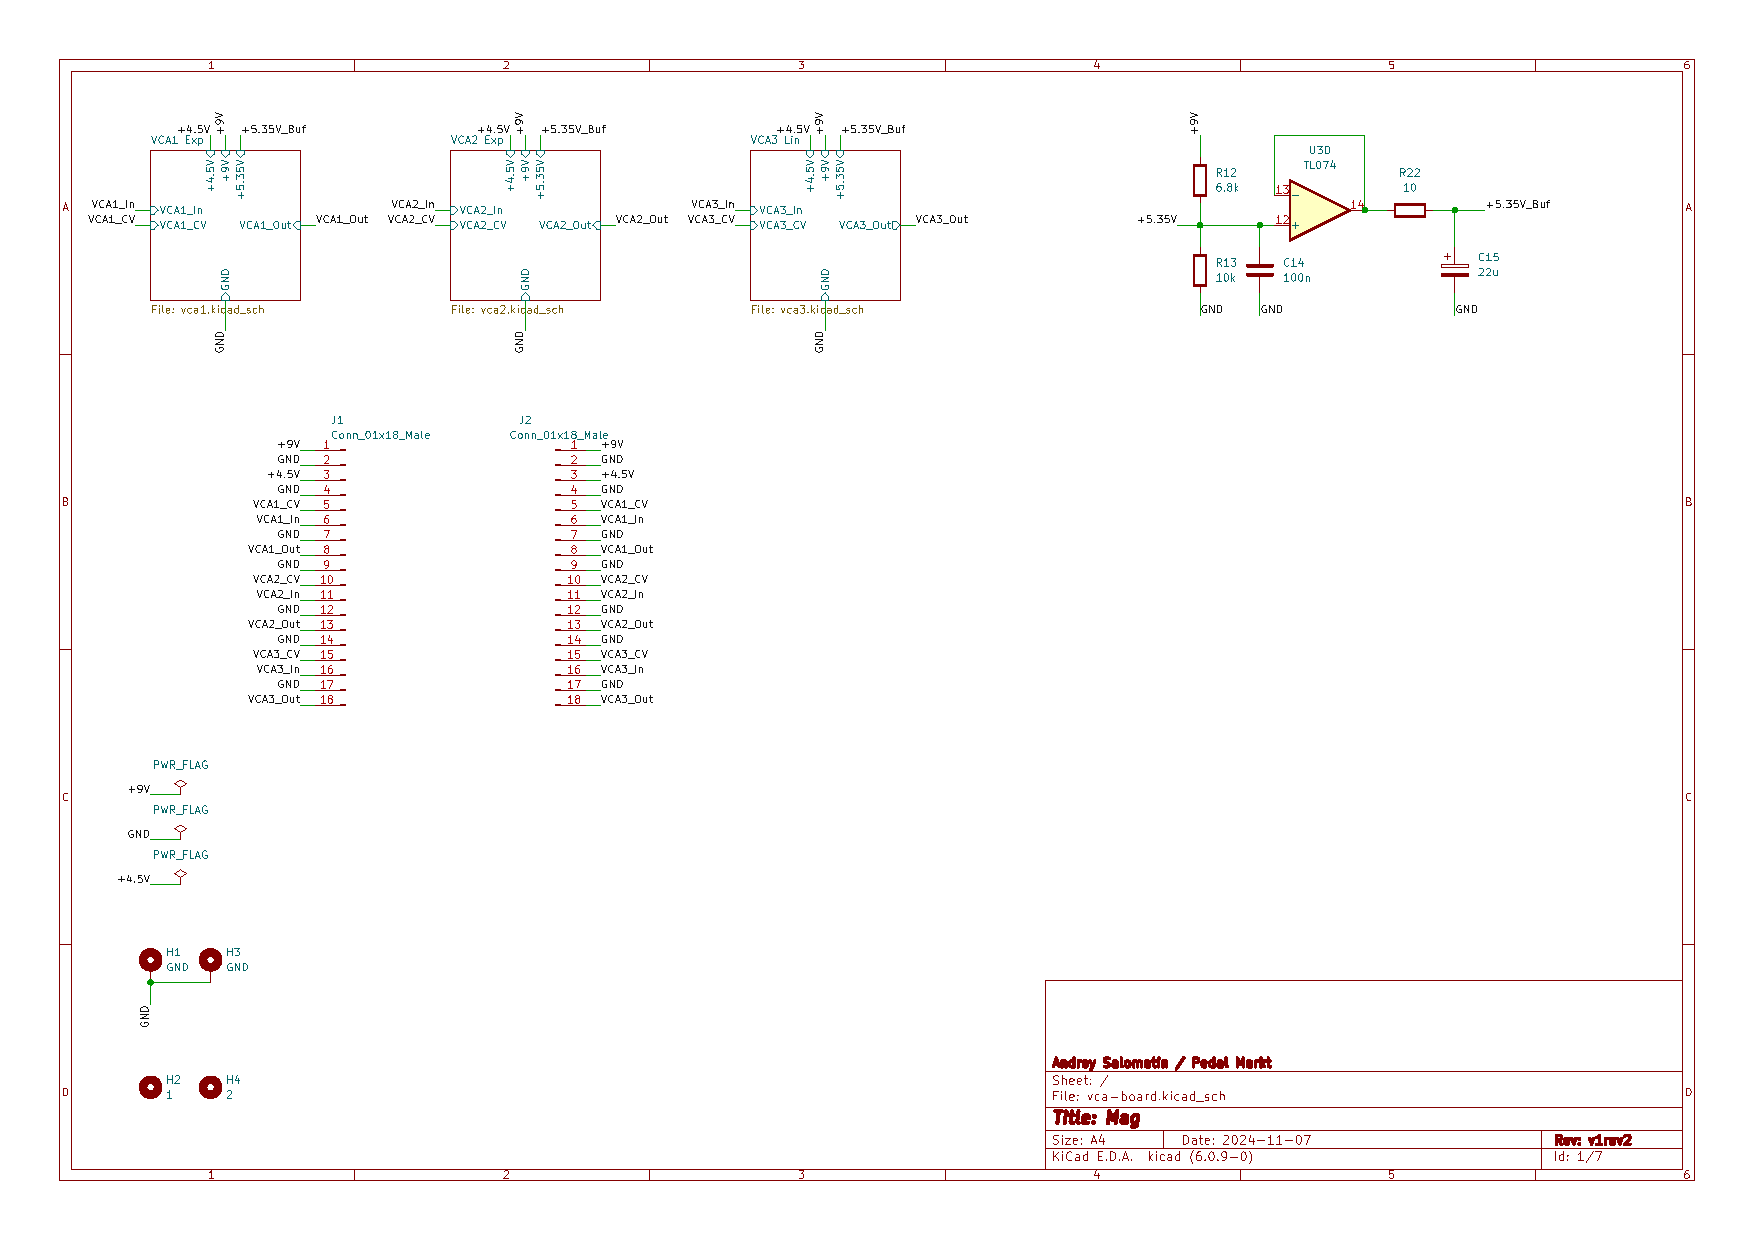
\includepdf[pages=-,landscape=true]{include/mag-v1rev2.pdf}

\section{Demod}\label{sec:demod}

Demod is an envelope follower and peak detector with
variable threshold. All outputs of demod are positive
relative to the virtual ground reference of \SI{4.5}{V}.

The board consists of a rectifier (Rect output) going into
both a low-pass filter (for the Follower output) and a
peak detector (for the peak output).


\begin{itemize}
  \item Schematic PDF:
    \href{https://github.com/flpvsk/pedalmarkt-docs/tree/main/elements2-modulation-docs/include}{GitHub}

  \item KiCad project:
    \href{https://github.com/flpvsk/pt-workshop/tree/main/follower-board}{GitHub}
\end{itemize}

\pagebreak

\begin{table}[h!]
  \caption{Demod Pinout}
  \centerline{
    \begin{tblr}{
      hlines,
      vlines,
      rows={ht=1.2em},
      row{1}={bg=gray3,fg=white},
      colspec={cccX[l]}
    }
      \textbf{Pin}
      & \textbf{Name}
      & \textbf{Type}
      & \textbf{Description}
      \\
      1 & 9V0 & Pwr & \SI{9}{\V} power
      \\
      2 & GND & Pwr & Ground
      \\
      3 & 4V5 & Ref & \SI{4.5}{\V} reference
      \\
      4 & In & In & Input signal, AC-coupled
      \\
      5 & GND & Pwr & Ground
      \\
      6 & Rect & Out & Rectified signal
      \\
      7 & Follower & Out & Envelope follower
      \\
      8 & GND & Pwr & Ground
      \\
      9 & Thresh & In & Threshold for the peak detector
      \\
      10 & Peak & Out & Peak detector output
      \\
      11 & GND & Pwr & Ground
    \end{tblr}
  }
\end{table}

\pagebreak

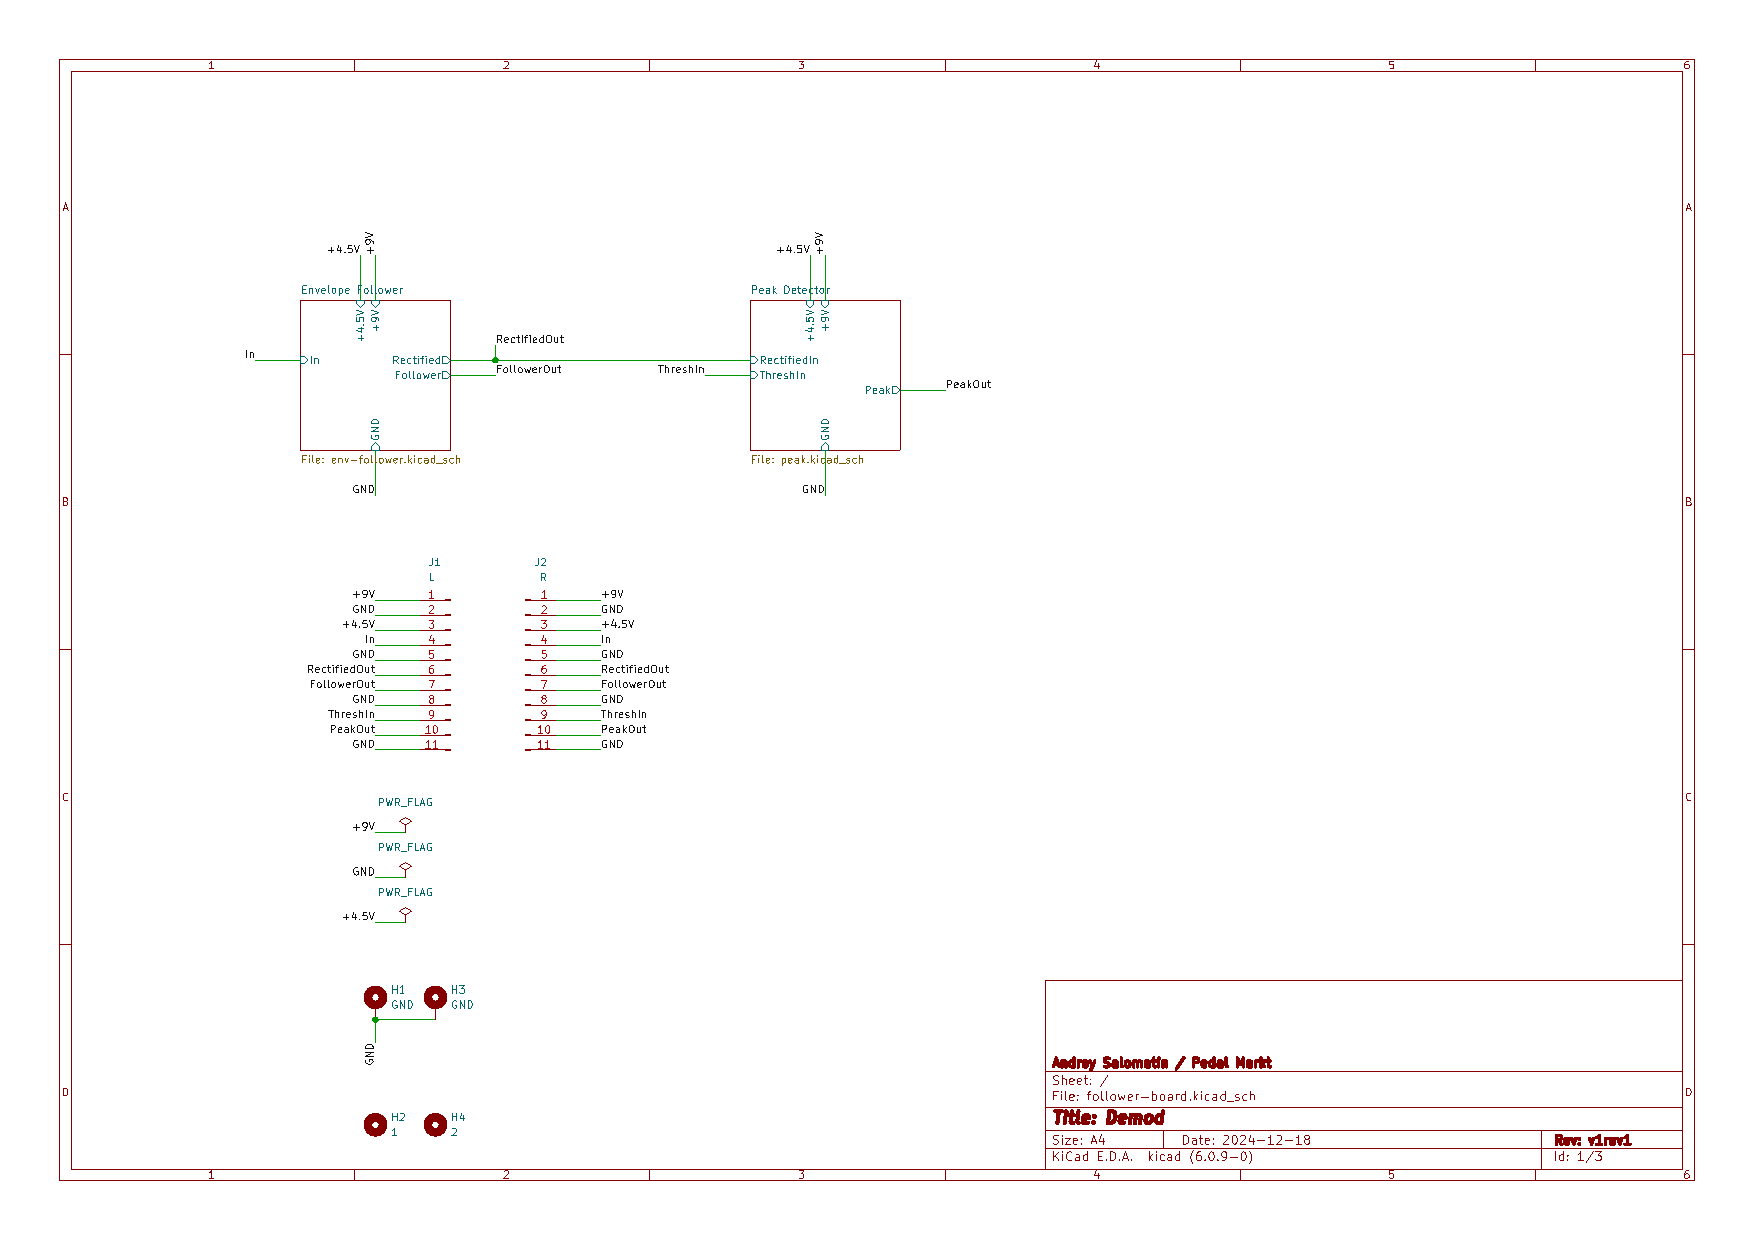
\includepdf[pages=-,landscape=true]{include/demod-v1rev1.pdf}
\end{document}
